% ============================================================================
%  Chapter 4. Results. \input file for main_msu.tex; requires booktabs, float,
%  graphicx, amsmath, natbib and \apanote. Bibliography: accord/thesis/refs.bib
%
%  PROVENANCE RULE: every numeric value below is registered in
%  results/accord/VERIFIED_FACTS.json, reported at the precision of that
%  register or rounded to four decimal places. A quantity the register does not
%  contain is stated qualitatively instead. Nothing is carried forward from an
%  earlier draft.
% ============================================================================

\chapter{Results}
\label{ch:results}

This chapter reports the measurements taken at each stage of the pipeline, one
section per research question, in the order the stages run: the reading a
competent evaluation would produce, the control designed to separate that
reading from an artifact of measurement, and what the control returned.

Three evaluation sets appear throughout and they are not interchangeable.
Table~\ref{tab:denoms} fixes them. Every metric below carries its denominator, and
a quantity that is a ratio of two registered counts is written as that ratio, for
example $12/253$.

\begin{table}[H]
\caption[The three evaluation sets]{The three evaluation sets used in this chapter.}
\centering
\small
\begin{tabular}{lrrrl}
\toprule
\textbf{Set} & \textbf{$n$} & \textbf{Positives} & \textbf{Negatives} &
\textbf{Definition} \\
\midrule
$G_{299}$ & 299 & 12 & 287 & all annotated pairs, ambiguous counted negative \\
$G_{253}$ & 253 & 12 & 241 & non-ambiguous pairs, ambiguous dropped \\
$G_{134}$ & 134 & 6  & 128 & Rule 3 and Rule 4 stratum, defect free \\
\bottomrule
\end{tabular}
\apanote{$G_{299}$ is all annotated pairs; $G_{253}$ excludes the ambiguous pairs; $G_{134}$ is the defect-free stratum from the control report. The 46 ambiguous pairs are the difference between the two negative counts, $287 - 241$. $G_{134}$ is a subset of $G_{299}$ and holds half of the 12 confirmed contradictions.}
\label{tab:denoms}
\end{table}

A spread reported as $\pm$ or as SD in this chapter is a standard deviation
across three seeds, not a standard error and not a confidence interval
(Section~\ref{sec:m-stats}). That standard deviation follows two conventions, because the underlying
artifacts use two: the decontamination
sources compute it at $\mathrm{ddof} = 0$, the population convention, and the
control, convergence and ablation sources compute it at $\mathrm{ddof} = 1$,
the sample convention. Each table below states which convention its own spreads
use, and no spread computed under one convention is compared against one
computed under the other.

\section{Candidate Generation}
\label{sec:res-rq1}

Can rule-based mining over paired notes yield a candidate pool with usable
precision? No. More useful is that the pool's measured precision bounds the
validity of the annotation exercise rather than the pipeline's quality.

\subsection{The pool and its base rate}

A board-certified pharmacist annotated 299 candidate pairs: 12 contradictions,
241 not contradictions, 46 ambiguous. The base rate is $12/299$ on $G_{299}$,
$12/253$ on $G_{253}$ and $6/134$ on $G_{134}$. The majority-class baseline has
average precision $0.0401$ on $G_{299}$ and $0.0448$ on $G_{134}$, the no-skill
lines for every average precision in this chapter. A pool at a base rate near four percent is not itself a failure,
because rule-based mining is a recall device and a low-precision pool is its
expected output. What fails is what the precision figure is then used to justify.

\subsection{Per-rule yield and precision}

The candidate pool itself is dominated by one rule: of the 1,978 post-prefilter candidates,
886 come from Rule 1, 202 from Rule 2, 520 from Rule 3 and 370 from Rule 4
(Section~\ref{sec:m-candidates}), so Rule 1 alone supplies close to half the pool. Pharmacist
precision, measured on the 299-pair gold sample, does not track that share. Table~\ref{tab:rule-precision}
gives the size of each rule's gold stratum, the pharmacist's true-positive rate on it, and ACCORD's
predicted-positive rate on the same rows.

\begin{table}[H]
\caption[Per-rule precision and predicted-positive rate]{Per-rule gold stratum size, pharmacist precision, and ACCORD's predicted-positive rate.}
\label{tab:rule-precision}
\centering
\small
\begin{tabular}{lrrr}
\toprule
\textbf{Rule} & \textbf{$n$} & \textbf{Pharmacist precision} & \textbf{ACCORD predicted positive} \\
\midrule
1, direct action conflict & 134 & 2.24\% & 97.01\% \\
2, drug class conflict    & 31  & 9.68\% & 96.77\% \\
3, dosage conflict        & 79  & 5.06\% & 97.47\% \\
4, discharge-side absence  & 55  & 3.64\% & 74.55\% \\
\bottomrule
\end{tabular}
\apanote{The four strata sum to 299. The ACCORD column is the contaminated released run of Table~\ref{tab:marginal} ($134 \times 0.9701 + 31 \times 0.9677 + 79 \times 0.9747 + 55 \times 0.7455 \approx 278$). A rule is a mining mechanism, not a clinical category: the pharmacist's failure-mode coding of the 12 confirmed contradictions returns 7 omissions, 3 dosage conflicts, 1 drug substitution and 1 class conflict, spread across all four rules rather than confined to Rule 4, whose gold stratum contains 2 of the 12.}
\end{table}

Table~\ref{tab:rule-precision} shows pool volume and hit rate moving in
opposite directions: Rule 2 has the highest pharmacist precision despite the
smallest gold stratum and pool share, and Rule 1 the lowest despite the
largest, so no single rule accounts for the pool's overall base rate.
ACCORD's predicted-positive rate is insensitive to that more-than-fourfold
spread in true precision across Rules 1 through 3, and drops only for Rule 4,
the rule with no discharge-side mention to score, consistent with the
calibration failure of Section~\ref{sec:res-rq2} rather than with
rule-sensitive discrimination. Combined, Rules 3 and 4 account for 134 of the
299 pairs and 6 of the 12 confirmed contradictions, so the positives are
spread across the rule set rather than concentrated in one rule.

Grouping by mechanism rather than by rule number, Rules 1 and 2 together
account for $165$ pairs with $6$ positives, a rate of $0.0364$; Rules 3 and 4 together account for
$134$ pairs with $6$ positives, a rate of $0.0448$. A Fisher exact test on that $2 \times 2$ table
gives an odds ratio of $0.805$ at $p = 0.7725$, achieved power is $0.0576$, and the smallest
absolute rate difference detectable at $80\%$ power is $0.0895$, more than twice the overall base
rate. The two mechanism groups are indistinguishable at this sample size, which is not the same as equal.
The per-rule reading stops at Table~\ref{tab:rule-precision}. A ranking statistic computed inside a
single rule would rest on a handful of confirmed positives with no committed interval to bound it,
so none is reported for a rule on its own.

\subsection{The exemplar selection defect}
\label{sec:r-exemplar}

Each candidate reached the annotator as one nursing sentence paired with one
discharge sentence. For the two action-conflict rules the discharge sentence was
taken from the first row of the matched-mention frame rather than the row
carrying the conflict that triggered the candidate. For a large minority of
action-conflict candidates the annotator therefore judged a sentence pair that
did not exhibit the conflict the prompt asserted was present.

Two measurements of how often the defect fired exist on the $165$ pooled Rule 1
and Rule 2 candidates, and they disagree, so both are reported. The first
reconstructs the exemplar from a mentions-table snapshot, calibrated against
what the pharmacist actually saw at $0.8934$ nursing-side and $0.9508$
discharge-side fidelity, not perfectly, because Section~\ref{sec:m-exemplar}
establishes that the exact original row order cannot be recovered: 137 of the
165 candidates resolve, 28 do not, and among the 137, 65
carried a discharge sentence that did not exhibit the conflict, a wrong rate
of $0.4745$. The second uses
a true key join instead of a reconstruction, exact where it applies but
applying to far fewer rows: only 23 of the 165 candidates carry a usable join
key, and on that subset the exemplar is correct on all 23, a wrong rate of 0.
If the reconstruction's rate of $0.4745$ were the true
rate and joinability were independent of correctness, the probability of drawing $23$
joinable rows and finding all $23$ correct would be $0.5255^{23}$, which is about
$4$ in ten million. The two measurements are therefore not two ends of one interval.
They are mutually exclusive unless joinability is strongly confounded with
correctness, and that confound is the load-bearing assumption behind keeping both
numbers. It is plausible on its face: a row carries a usable join key when
the pipeline's own bookkeeping about it was intact, the bookkeeping the
selector defect corrupts. That assumption is stated here, left untested, and
an attempt to test it is reported as inconclusive rather than as a result.

The two-by-two is stark: of the $23$ rows the key join resolves, $23$ are correct,
against $72$ correct and $65$ wrong among the $137$ the reconstruction resolves.
It is not a test of association: correctness for the $23$ was assessed by
the key join and for the $137$ by the reconstruction, so no row is measured by
both. The hypothesis such a table would reject is the conjunction of two claims,
that joinability is unrelated to correctness and that the two instruments share
an error rate; the second is already denied, since the reconstruction's
fidelity is calibrated against what the pharmacist saw while the key join is
asserted exact. A comparison across instruments of unequal known fidelity cannot
attribute its difference to the thing being studied. The rival reading generates
the same table and points the other way: rows that reconstruct badly may be
called wrong by the reconstruction rather than by the defect, making joinability
a proxy for reconstructability and $0.4745$ the artifact.

So the $23$ key-joined rows are not a random subsample of the $165$, and that is the whole of
what the table supports. It is reported without a $p$ value and is not a member of the
hypothesis family Section~\ref{sec:r-multiplicity} enumerates; a $p$ value was briefly
attached and counted there, and C90 records why both were wrong. The confound remains
unfalsifiable from the retained artifacts, which is a weaker and more accurate position than a
confirmation. One of these two numbers is still wrong and this thesis still does not know
which. Neither is discarded, and neither should be quoted alone. A
separate join, across all four rules rather than Rule 1 and 2 alone, matches
the $299$-row annotated sample to the rebuilt candidates table on $35$ rows;
that is a different operation with a different denominator, not a third
reading of the same exemplar-correctness question.
Figure~\ref{fig:exemplar} in Chapter~\ref{ch:intro} draws the mechanism the two
measurements are measuring. The rate at which the trigger-set slot and the
positionally indexed slot actually disagreed on the Rule 1 and Rule 2 gold
stratum ranges from $0$ to $0.4745$ depending on measurement, and a rate over a
population does not belong welded to a picture of a single case, so the figure
carries no number.

The measured consequence does not depend on that rate. Rules 3 and 4 cannot
exhibit the defect: Rule 3 selects the maximum-difference dose pair, and Rule 4
has no discharge sentence to select, because the drug is absent from the
discharge summary by construction. That yields $G_{134}$, and
Section~\ref{sec:res-rq4} reports two scores on that stratum: the defect-free
control model's, and ACCORD's contaminated released run rescored on the same
pairs. What it does not report is the decontaminated ACCORD ensemble on
$G_{134}$, because no per-pair score from the decontaminated retrain was
retained for those rows. The restriction does not move the conclusion and it
widens the intervals, as a stratification down to 6 positives at a minimum
detectable AUROC of $0.8058$ has to. The figure this defect bounds is an upper
bound on annotation validity, not an estimate of pipeline quality, and the
direction of the bias is unknown.

\section{Weak Supervision}
\label{sec:res-rq2}

Can an LLM weak labeller substitute for expert annotation at this base rate? No.
Every local labeller tested over-calls on the same pairs, by roughly fifteen to
twenty-four times the confirmed rate at eight billion parameters, already
enough review burden to matter for anyone judging how much of a pipeline
like this still needs a human check. Whether that multiplier falls
further at frontier scale was tested through a hosted API and the result is
withdrawn (Section~\ref{sec:r-frontier}); this chapter does not establish
whether the failure attenuates with capability or bottoms out at eight billion
parameters.

\subsection{The marginal}

On the 299 annotated pairs the weak labeller called 261 pairs contradictions and
the pharmacist called 12. Table~\ref{tab:marginal} puts the three marginals on
the one denominator where all three were recorded. Weak supervision of this kind
is defended on the grounds that the noise averages out \citep{ratner2017snorkel},
and that defence assumes noise conditionally independent across sources given the
label; one source whose error is a shifted marginal falls outside the regime.

\begin{table}[H]
\caption[Predicted-positive counts by source]{Predicted-positive counts on the 299 annotated pairs.}
\centering
\small
\begin{tabular}{lrl}
\toprule
\textbf{Source} & \textbf{Called contradiction} & \textbf{Denominator} \\
\midrule
Pharmacist (gold)                  & 12  & 299 \\
Llama 3 8B weak labeller           & 261 & 299 \\
ACCORD, released per-pair decision & 278 & 299 \\
\bottomrule
\end{tabular}
\apanote{The ACCORD decision column is three-valued; 15 rows carry the value \emph{ambiguous}. The 261 and the 278 count two different columns produced by two different systems on the same 299 rows and are not two readings of one quantity. The ACCORD row is the contaminated released run; the decontaminated retrain appears in Section~\ref{sec:res-rq4}.}
\label{tab:marginal}
\end{table}

$261$ against $12$, on identical inputs, is the finding.
\citet{pangakis2023validation} argue that an automated annotation procedure must
be validated against human labels on the same items; those items existed
before the labelling run, and the comparison was not made.

Three local 8B labellers were each run over the pool and the gold set, and the
over-calling ratio, the positive rate divided by the gold base rate of
$0.0401$, was measured for all three with zero unparseable responses.
Table~\ref{tab:overcalling} carries every over-calling ratio this chapter
reports, together with the positive rate and the count each rate is measured
on, so measurements taken on different sets are not mistaken for readings of
one quantity.

\begin{table}[H]
\caption[Over-calling ratios by labeller and evaluation set]{Every over-calling ratio this chapter reports on the candidate pool and on $G_{253}$, by labeller, evaluation set, positive rate, and the count the rate is measured on.}
\label{tab:overcalling}
\centering
\small
\begin{tabular}{@{}p{1.55in}p{1.15in}rrr@{}}
\toprule
\textbf{Labeller} & \textbf{Evaluation set} & \textbf{Positive rate} & \textbf{Ratio to $0.0401$} & \textbf{$n$} \\
\midrule
\texttt{llama3:8b}     & Candidate pool                    & 0.9470 & 23.5959 & 1,679 \\
\texttt{llama3:8b}     & $G_{299}$, gold set                & 0.9532 & 23.75   & 299   \\
\texttt{granite3.3:8b} & Candidate pool                    & 0.7219 & 17.9863 & 1,679 \\
\texttt{granite3.3:8b} & $G_{299}$, gold set                & 0.7425 & 18.5    & 299   \\
\texttt{qwen3:8b}      & Candidate pool                    & 0.6349 & 15.8196 & 1,679 \\
\texttt{qwen3:8b}      & $G_{299}$, gold set                & 0.6187 & 15.4167 & 299   \\
Llama 3, deployed weak labeller & Candidate pool & $1425/1679$ & 21.1473 & 1,679 \\
\bottomrule
\end{tabular}
\apanote{Each ratio divides a positive rate by the unrounded $12/299$ gold base rate, so recomputing from the printed $0.0401$ will not reproduce these ratios exactly. The first six rows are three local labellers on the candidate pool and the gold set; the seventh, the deployed weak labeller, differs by prompt (Section~\ref{sec:m-weak}). The $15.8196$ to $23.5959$ range quoted elsewhere is this across-model range on the pool alone. A frontier-scale labeller run on this pool through a hosted API is withdrawn (Section~\ref{sec:m-ethics}) and does not appear here.}
\end{table}

Every ratio measured is well above 1, so no local 8B labeller tested is close
to calibrated at this base rate.

A ratio of marginals says how often a labeller calls a positive and nothing
about whether it calls the right ones, and this chapter measures the
deployed weak labeller only that way, a property of the
labelling policy rather than a gap in the analysis. On the joined rows it
emits a positive for $0.9017$ of them against a confirmed rate of $0.0474$;
at that marginal, perfect agreement with the pharmacist is arithmetically
unreachable: holding the flagged count fixed and placing every confirmed case
inside it, the largest Matthews correlation any thresholded label could
express is $0.0768$. The supervision the detector was trained on could not
have carried more than that, whatever the labeller knew, and that ceiling
follows from two counts on the joined rows, before any training: it is the mechanism
behind the detector's own degeneracy, a model fit to labels emitted at a
marginal of $0.9$ inheriting the marginal, as
Table~\ref{tab:operating} shows.

What cannot be measured is the labeller's own agreement, reported as a
negative result rather than omitted. The weak-label file and the gold file
share no identifying column, so any pair-level comparison is a reconstruction
through a nursing-side key, matching on rule at $95$ of $299$ against $94.3$
expected by chance; on that reconstruction the correlation is $0.0117$. Under
a random re-alignment of the same labels, which leaves the marginal untouched,
the observed correlation sits at the $0.6648$ point of the random-join
distribution, so two thirds of scrambled joins do better: the reconstruction
cannot distinguish a labeller at chance from an arbitrary labeller joined
badly, and no agreement statistic for this labeller is recoverable from the
retained artifacts.

The over-calling ratios are not undercut by this: they measure what they
claim, and the ceiling explains why a high positive rate on a rare event caps
what any downstream model can inherit. Nor does this section adjudicate
whether the task or the pipeline fails, since a labeller at chance is what
both readings predict; an analysis that might have separated the two readings
was run through a hosted service and is withdrawn along with the run that
produced it (Section~\ref{sec:r-frontier}), so this thesis does not establish
whether the task is unlearnable at this sample size from that direction
either.

\subsection{Whether a stronger labeller removes it}

If the over-calling were an artifact of a small open-weights model, a stronger
labeller would remove it. This question was put to a frontier-scale labeller
through a hosted API, and that run is withdrawn along with everything computed
from it (Section~\ref{sec:r-frontier}); what a frontier-scale model does on
this pool is therefore not established anywhere in this thesis. What the local
labellers alone support is narrower: every one of them measured on this pool
over-calls, and Table~\ref{tab:systems253} shows this project's own detector and
its evaluation baseline doing the same thing.

\begin{table}[H]
\caption[Per-pair calls on the core evaluation set]{Per-pair calls on the 253 non-ambiguous pairs.}
\centering
\small
\begin{tabular}{lrrrrrr}
\toprule
\textbf{System} & \textbf{TP} & \textbf{FN} & \textbf{FP} & \textbf{TN} &
\textbf{Precision} & \textbf{Recall} \\
\midrule
ACCORD at $\tau = 0.5$         & 11 & 1 & 223 & 18  & 0.0470 & 0.9167 \\
Llama 3 8B evaluation baseline & 11 & 1 & 231 & 10  & 0.0455 & 0.9167 \\
\bottomrule
\end{tabular}
\apanote{On $G_{253}$, 12 positives and 241 negatives. The last row is a separately prompted Llama 3 8B evaluation run and is \emph{not} the weak-supervision labeller of Table~\ref{tab:marginal}, whose own calls on these pairs differ. The ACCORD row is the contaminated released run, whose recall of 11 of 12 no decontaminated seed reaches; it is kept only because its per-pair calls are the committed ones.}
\label{tab:systems253}
\end{table}

The two systems at recall $0.9167$ (Table~\ref{tab:systems253}) reach it the
same way, by predicting the positive class for almost every pair. Recall alone
is the least informative statistic, because a constant-positive
predictor attains recall $1.0$ by construction at precision exactly equal to
the base rate of whichever set it is scored on, and that predictor, the
mining rules treated as the whole system, is the floor the two rows
have to clear: both sit below $12/253$. Neither gap is tested, because no
significance test for a margin this size is computed anywhere in this thesis;
what the two rows support without a test is that this thesis's own detector
and its evaluation baseline sit at or fractionally under the precision the
rules alone would reach for free.

\subsection{The public-text replication}

The same three local models were run over a public-text contradiction sweep on
SNLI in which the true positive rate was varied and each model's marginal recorded
at every setting, with the same greedy decoding at temperature zero but with
generic sentence-pair prompts, not the recovered clinical prompt. The mismatch on
public text is far smaller than the mismatch here, and it is not consistently in
one direction.

Figure~\ref{fig:prevalence-response} shows the sweep in full. The maximum over-calling ratio measured across it, three models, two prompts and four
prevalence levels on SNLI, is $3.5000$, reached by \texttt{llama3:8b} under the bare prompt at 2
percent true prevalence; the next highest is $3.4000$, the same model and prompt at 5 percent
prevalence. Both sit well below the
$15.8196$ to $23.5959$ range of pool over-calling ratios Table~\ref{tab:overcalling} records above
in this section. The magnitude of the failure is therefore not a general property of an
instruction-tuned labeller asked for a rare positive class. Neither is its direction: most
public-text settings under-call, \texttt{qwen3:8b} never over-calls there, and because the
sweep changed the prompt and the kind of negative as well as the domain, it cannot say which
of the three produces the clinical gap.

Attributing the gap's size to the pool's base rate rather than to the model
would require a frontier-scale labeller on the clinical pool, the cell the
design does not contain (Section~\ref{sec:r-frontier}): with scale held fixed
across all three local labellers, a difference between the clinical pool and
the public-text sweep could only be attributed to the pool, which is not a
conclusion this design licenses. What survives is narrower: an over-calling
multiplier reported without naming both the base rate it was measured against
and the model that produced it is uninterpretable, and no claim is licensed
about any model not tested here or about clinical text beyond this pool.

\begin{figure}[!t]

\centering
\caption[Labeller response to prevalence]{Weak-labeller positive rate against
true prevalence for three open-weight models under two prompt conditions. The
diagonal is perfect calibration; the tinted wedge is over-prediction. Wilson
intervals from the sweep's decision counts. The filled point is the deployed
weak labeller at this thesis's clinical operating point.}
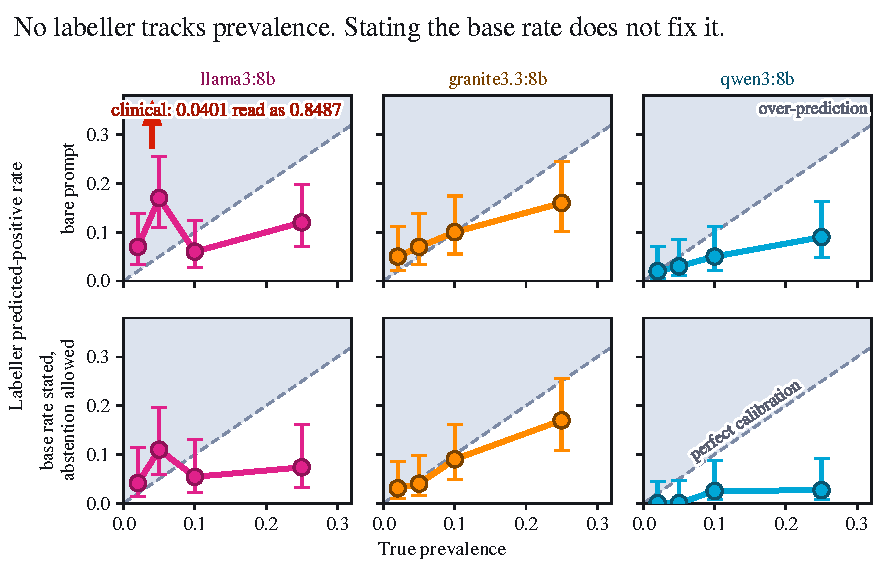
\includegraphics[width=0.98\linewidth]{figures/fig-prevalence-response.pdf}
\label{fig:prevalence-response}
\end{figure}

\subsection{The cell the design did not contain}
\label{sec:r-frontier}

Section~\ref{sec:m-control-rq2} states the condition this control was built to
decide: if over-calling is a property of one model it will not survive a change of
model, and if it is a property of the task presentation it will. The replication
changed the model three times and the domain once, and never changed the scale:
all three local labellers are eight-billion-parameter instruction-tuned models, so
the design is a two-by-two in domain and prevalence with capability held fixed, and
the cell it does not contain is a frontier-scale labeller on the clinical pool.

That cell was filled by transmitting MIMIC-III sentence pairs to hosted API
services, Claude Sonnet 5 and Claude Haiku 4.5 through the Anthropic API and
Llama 3 70B and Llama 3 8B through AWS Bedrock. PhysioNet's guidance on the use
of MIMIC data with third-party LLM services withdrew the safe-harbour list those
runs relied on (Section~\ref{sec:m-ethics}), so every one of those runs, and every
number, table, and figure computed from one, is withdrawn from this thesis. That
includes the capability ladder and the frontier discrimination table.
Whether a frontier-scale labeller removes the over-calling this chapter measures
at eight billion parameters is therefore not established here; the local-only
finding of Section~\ref{sec:res-rq2} is the one this thesis can support.

\subsection{The marginal feasibility gate}
\label{sec:r-feasgate}

Before a labeller's agreement with the pharmacist is read as evidence, its own
marginals already fix how much agreement it could possibly have shown. Holding
the confirmed count and the flagged count fixed and placing every confirmed
case inside the flagged set gives the best table those two marginals permit: a
Matthews correlation ceiling, a kappa ceiling, and the smallest one-sided
hypergeometric $p$ the labeller's own margins could return against the
pharmacist's labels. That floor $p$ is a precondition rather than a result: it
is computable before a single pair is scored, and it says whether the test
that follows could have rejected the null at all.

This bounds a thresholded decision only, and the qualification is not
optional, because the unqualified claim is false. A labeller that emits a
continuous score is not bounded this way, because the threshold that turns a
score into a flag can be swept; a model that flags most of a pool at one
threshold can still rank the pool well at another. Everything below is a
statement about labeller-and-prompt configurations in this thesis that emit a
hard label on this pool, not about a score-emitting model. One score-emitting model was measured,
under a rule registered before the run (C98): \texttt{granite3.3:8b}'s first-token
log-odds of a contradiction, graded across the $253$ non-ambiguous pairs, reaches
an AUROC of $0.5467$ (one-sided Mann-Whitney $p = 0.2934$), below the $0.7355$
this evaluation can resolve. Sweeping its threshold does not rescue it.

Table~\ref{tab:feasgate} and Figure~\ref{fig:ceiling} apply the gate to every
local labeller-and-prompt configuration this chapter scores against the
pharmacist on this pool: \texttt{granite3.3:8b} and \texttt{llama3:8b},
zero-shot and few-shot, each on both $G_{253}$ and $G_{299}$, four
configurations on two nested bases, eight rows. Two of the four,
\texttt{llama3:8b} at both prompts, could not have rejected the null at
$0.05$ on either basis before scoring a single pair, because the smallest $p$
their own marginal permits already exceeds $0.05$. Two of the four sit
exactly on their marginal-implied ceiling on both bases,
\texttt{granite3.3:8b} zero-shot and \texttt{llama3:8b} few-shot: their
observed agreement equals the best any labeller at that flag rate could
achieve, so no retuning of that labeller at that marginal could have moved it
further. The two sets overlap on \texttt{llama3:8b} few-shot, which sits on
its ceiling while unable to reject the null, the least a labeller can show at
that marginal; \texttt{granite3.3:8b} zero-shot sits on its ceiling while
rejecting the null, the most that marginal permits.

The table also carries every other hard-label marginal this chapter prints,
whether or not this project ever joined it to the pharmacist's labels row by
row: the inclusion rule is every hard-label marginal this chapter prints.
That adds five rows: the deployed weak labeller (Table~\ref{tab:marginal}),
the Llama 3 8B evaluation baseline on $G_{253}$ (Table~\ref{tab:systems253}),
and the three baseline-prompt local labellers on $G_{299}$
(Table~\ref{tab:overcalling}). The evaluation baseline is the one of these
scored row by row, and its observed MCC is printed; the other four read
\emph{not scored}. The baseline and the \texttt{llama3:8b} baseline-prompt row
are one configuration on two nested bases, so the table covers eight
configurations, not nine. Four could not have rejected the null at $0.05$ at any
outcome, all \texttt{llama3:8b}. The check was added after the hosted results
were withdrawn and is reported here as a post hoc precondition.

\begin{table}[H]
\caption[The marginal feasibility gate, every hard-label marginal this
chapter prints]{The marginal feasibility gate applied to every hard-label
labeller marginal this chapter prints: scored where this project joined the
labeller to the pharmacist row by row, unscored where only the marginal
survives.}
\centering
\footnotesize
\begin{tabular}{llrrrrrl}
\toprule
\textbf{Labeller} & \textbf{Basis} & \textbf{Flag rate} & \textbf{Obs.\ MCC} &
\textbf{Ceil.\ MCC} & \textbf{Ceil.\ $\kappa$} & \textbf{Floor $p$} & \textbf{Verdict} \\
\midrule
\texttt{granite3.3:8b}, few-shot  & $G_{253}$ & 0.6957 & 0.0668 & 0.1476 & 0.0426 & 0.0114 & Could reject \\
\texttt{granite3.3:8b}, few-shot  & $G_{299}$ & 0.7023 & 0.0586 & 0.1331 & 0.0348 & 0.0131 & Could reject \\
\texttt{granite3.3:8b}, zero-shot & $G_{253}$ & 0.7391 & 0.1326 & 0.1326 & 0.0345 & 0.0242 & Could reject, at ceiling \\
\texttt{granite3.3:8b}, zero-shot & $G_{299}$ & 0.7492 & 0.1183 & 0.1183 & 0.0276 & 0.0290 & Could reject, at ceiling \\
\texttt{llama3:8b}, few-shot      & $G_{253}$ & 0.9447 & 0.0540 & 0.0540 & 0.0058 & 0.4971 & Could not reject, at ceiling \\
\texttt{llama3:8b}, few-shot      & $G_{299}$ & 0.9398 & 0.0518 & 0.0518 & 0.0053 & 0.4679 & Could not reject, at ceiling \\
\texttt{llama3:8b}, zero-shot     & $G_{253}$ & 0.8735 & 0.0290 & 0.0849 & 0.0143 & 0.1898 & Could not reject \\
\texttt{llama3:8b}, zero-shot     & $G_{299}$ & 0.8729 & 0.0269 & 0.0780 & 0.0121 & 0.1894 & Could not reject \\
\midrule
Llama 3, deployed weak labeller       & $G_{299}$ & 0.8729 & not scored & 0.0780 & 0.0121 & 0.1894 & Could not reject \\
Llama 3 8B eval.\ baseline, prompted once & $G_{253}$ & 0.9565 & $-0.0436$ & 0.0476 & 0.0045 & 0.5795 & Could not reject \\
\texttt{llama3:8b}, baseline prompt      & $G_{299}$ & 0.9532 & not scored & 0.0453 & 0.0041 & 0.5562 & Could not reject \\
\texttt{granite3.3:8b}, baseline prompt  & $G_{299}$ & 0.7425 & not scored & 0.1204 & 0.0286 & 0.0259 & Could reject \\
\texttt{qwen3:8b}, baseline prompt       & $G_{299}$ & 0.6187 & not scored & 0.1605 & 0.0502 & 0.0027 & Could reject \\
\bottomrule
\end{tabular}
\apanote{Ceiling MCC and ceiling $\kappa$ hold every confirmed case inside the
flagged set. Of the five rows below the rule only the evaluation baseline was
scored row by row; the others read \emph{not scored}. Floor $p$ is the smallest one-sided hypergeometric $p$ the marginal
allows (Section~\ref{sec:r-multiplicity}), a precondition rather than a test
unless observed MCC equals ceiling MCC, where it is also the exact test
observed. Basis is $G_{253}$ or $G_{299}$ (Table~\ref{tab:denoms}); every
cell is generated, none is typed.}
\label{tab:feasgate}
\end{table}

\begin{figure}[t]
\centering
\caption[The agreement ceiling a labeller's marginal imposes]{Largest Cohen's
kappa any thresholded labeller can reach against the pharmacist, as a function of
its positive rate on the $299$ gold pairs. The curve is an identity of the two
marginals, not a fit, so it carries no interval. Marked rows attain their own
ceiling. A labeller emitting a score is not bounded this way, because its
threshold can be swept.}
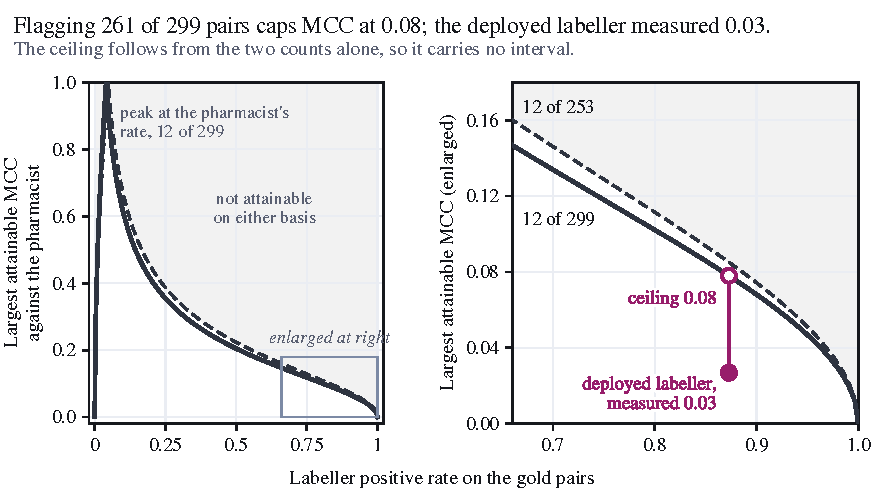
\includegraphics[width=0.98\linewidth]{figures/fig-ceiling.pdf}
\label{fig:ceiling}
\end{figure}

What the gate does not do is replace the discrimination tests reported
elsewhere in this chapter; it is read beside them, as a check on what a table
could have shown before it is read as showing it. A labeller whose floor sits
above the threshold, \texttt{llama3:8b} at both prompts here, was never going
to distinguish itself from chance at this marginal, and a labeller sitting on
its ceiling flagged every confirmed positive; at that flag rate it could not
have scored higher, whatever it otherwise knew about the pairs.

\subsection{What the false positives land on}
\label{sec:r-ambiguity}

Whether a labeller concentrates its false positives on the pairs the
pharmacist declined to call, rather than spreading them evenly across the
$287$ non-confirmed pairs, was tested by a one-sided Fisher exact test on flag
rate, ambiguous against clear-negative, replicated across labellers under two
prompts each. Four hosted labellers under two prompts each were tested this
way, eight tests in total; every one was run through the Anthropic API or AWS
Bedrock, so every odds ratio, every $p$ value, and the gradient itself are
withdrawn with the runs that produced them (Section~\ref{sec:r-frontier}). The
two local labellers were put to the same test: \texttt{granite3.3:8b} returns
an odds ratio of $1.2801$ at $p = 0.3110$ few-shot and $1.5505$ at $p = 0.1788$
zero-shot; \texttt{llama3:8b} returns $0.6476$ at $p = 0.8577$ few-shot and
$0.9841$ at $p = 0.6220$ zero-shot, none rejecting the null at $0.05$
(Section~\ref{sec:r-multiplicity}). This chapter therefore does not establish
that the ambiguous pairs are disproportionately flagged by any labeller
tested. The one confound that would have bounded any surviving reading, that an
odds ratio compresses toward $1$ as a labeller's marginal saturates, applies
to the local tests just reported as much as to the withdrawn ones.

\subsection{What the instability costs, and what it does not}
\label{sec:r-labelnoise}

A label-instability analysis was run on the frontier labeller's per-pair
draws, asking how much a Matthews correlation would move if individual labels
flipped at random. Every cell that analysis read from is a hosted-API result
and is withdrawn along with it (Section~\ref{sec:r-frontier}); no equivalent
instability bound is reported for a local labeller in this thesis, because the
open-weights runs were single deterministic draws under greedy decoding rather
than a resampled distribution over labels.

\section{Architecture}
\label{sec:res-rq3}

Do the purpose-built components contribute what they were credited with? No
component survives what a code audit finds. No randomisation control was run
on any of these three clinical components; what follows are audit findings,
not controls firing: one parameter is falsified as an initialisation artifact,
one metric is vacated by label leakage, and one module was never trained.

\subsection{One falsified, one vacated by leakage, one never trained}

\paragraph{Authority conditioning is an initialisation artifact.} The parameter
reported as converging to the clinical note hierarchy is initialised at $1.0$
for the discharge branch and $0.5$ for the nursing branch, the exact pair
reported as discovered by training. Across three seeds the discharge value
ends between $1.0024$ and $1.0047$, mean $1.0038$, and the nursing value ends
between $0.5070$ and $0.5084$, mean $0.5076$. Both parameters move a small
fraction of their initial value across seeds. Each sits on a branch that is
immediately normalised, which removes most of what a per-branch scalar can do
and drives its gradient towards zero.

\paragraph{The rule-type head is label leakage.} The rule identifier is written
into the model's input feature vector and predicted from the same forward pass,
one linear layer away, so the auxiliary task is a copy. Out-of-domain transfer is
the diagnostic that separates a copy from learned structure, because the leaked
feature survives transfer and the surface correlations do not. This belongs to
the documented family of shortcut learning \citep{geirhos2020shortcut,
zech2018generalization}; the checkable point is narrower, that an auxiliary head
whose target is derivable from its inputs is not an auxiliary task. In domain the
rule-type head reaches a macro $F_1$ of $0.9603$. Transferred without retraining
it collapses by more than an order of magnitude on both secondary cohorts, as
Table~\ref{tab:transfer} records. That is
reported as a descriptive non-portability
result rather than further evidence of leakage: the code-level argument above
is dispositive on its own, and a literal copy of the rule-identifier feature
would transfer perfectly, since the feature and target stay
identical in any domain. The collapse instead shows that the in-domain macro
$F_1$ reflects the correlation between that feature and this cohort's label
distribution rather than a verbatim copy of it, a correlation that does not
hold in the transfer cohorts.

\begin{table}[H]
\centering
\caption[Rule-type head under cohort transfer]{The rule-type head in domain and
transferred without retraining. No interval is committed for any of these three
values, so none is printed and none should be inferred; they are single
measurements on the candidate counts shown.}
\label{tab:transfer}
\begin{tabular}{lrr}
\toprule
\textbf{Cohort} & \textbf{Candidates} & \textbf{Macro $F_1$} \\
\midrule
Heart failure, training domain & 1,978 & 0.9603 \\
Sepsis                         &   775 & 0.0654 \\
Acute kidney injury            & 1,983 & 0.0595 \\
\bottomrule
\end{tabular}
\end{table}

\paragraph{Harm estimation was never trained.} The guideline bank is one randomly
initialised parameter matrix, there is no corpus and no retrieval step, and the
harm head does not appear in the training objective. Over the 299 annotated
pairs its output ranges from $0.3977$ to $0.6096$, a narrow band
consistent with an untrained scorer rather than a calibrated severity measure.
Its rank correlation against the pharmacist danger rating over all 299 pairs is
$\rho = -0.0001$, $p = 0.9991$. The
severity-ranking question was therefore not tested, and any null reported
against that head measures an untrained module rather than the underlying
question.

\subsection{Three controls that fired positively}

These controls run on a second system: a provenance-conditioned encoder trained with masked
language modelling, not the clinical contradiction detector whose numbers appear elsewhere in this
chapter.

\paragraph{A control task, a thesis-original alignment control, and locality alone.} Ten arms of a
shared additive attention bias were trained on masked language modelling over packed multi-document
bundles with segment order shuffled so role is decorrelated from position
(Section~\ref{sec:m-control-rq3}). Seven ran at three seeds each and are the matched comparison the
condition specifies; three ran at a single seed each, reported for completeness, not as
matched comparisons against the three-seed rows. Table~\ref{tab:ablation} reports the mean
validation loss, its seed spread where more than one seed exists, and the loss reduction against the
no-bias arm for all ten.

\begin{table}[H]
\caption[Ten-arm architecture ablation results]{Ten-arm architecture ablation, mean validation loss.}
\label{tab:ablation}
\centering
\small
\begin{tabular}{lrrrrr}
\toprule
\textbf{Arm} & \textbf{Mean val.\ loss} & \textbf{SD} & \shortstack[r]{\textbf{$\Delta$ vs.}\\\textbf{vanilla}} &
\shortstack[r]{\textbf{\% of segment-}\\\textbf{index gain}} & \textbf{Seeds} \\
\midrule
Global positions restored  & 4.5122 & n/a & +0.1567 & n/a     & 1 \\
Vanilla, no bias           & 4.3554 & 0.0085 & 0       & 0\%     & 3 \\
T5 relative position bias  & 4.1035 & 0.0029 & -0.2520 & 26.6\%  & 3 \\
Length-bucket roles        & 4.0174 & n/a & -0.3380 & 35.7\%  & 1 \\
Misaligned block bias      & 3.9109 & 0.0293 & -0.4445 & 46.9\%  & 3 \\
Random roles (shuffled)    & 3.8587 & n/a & -0.4967 & 52.4\%  & 1 \\
ALiBi distance bias        & 3.7435 & 0.0023 & -0.6119 & 64.6\%  & 3 \\
True role labels           & 3.5310 & 0.0076 & -0.8244 & 87.0\%  & 3 \\
Segment-index bias         & 3.4078 & 0.0225 & -0.9476 & 100\%   & 3 \\
Hard block mask, fixed     & 3.2772 & 0.0124 & -1.0782 & 113.8\% & 3 \\
\bottomrule
\end{tabular}
\apanote{Mean validation loss and its SD are given per arm, with the change against vanilla and its share of the segment-index arm's reduction, the largest gain among the three-seed arms; the share is undefined for the global-positions row, which increases loss relative to vanilla. Seed spreads on the seven three-seed rows run from $0.0023$ to $0.0293$ nats against effects from $0.2520$ to $1.0782$ nats, so every ordering among them is resolved well outside seed noise. The three single-seed rows carry no spread and are shown for completeness only.}
\end{table}

Two rows in Table~\ref{tab:ablation} are stated as a finding, not as a
control check run on the way to one. A hard block mask with zero trainable
parameters, fixed rather than learned, beats every learned attention-bias arm
in the table, including the segment-index bias it was built to bound. And an
arbitrary positional ordinal carrying no provenance meaning beats true
role labels. Neither result bears on the clinical contradiction detector or
its precision reported elsewhere in this chapter.

The control task in the
sense \citet{hewitt2019control} define it is the random-roles arm, which holds
the label alphabet fixed and randomises the mapping from tokens to roles; it
ran at a single seed, so no significance claim attaches to it, and true role
labels reduce the loss more than that randomisation does, a directional gap
consistent with role semantics contributing something real on this seed. A
second single-seed arm, roles collapsed to length buckets, points the same
direction. The segment-index arm is different in kind: it substitutes an
arbitrary ordinal position for role identity rather than randomising role
identity, so a win for it is a competing hypothesis about what the mechanism
exploits, not a control task in the \citet{hewitt2019control} sense and not
evidence that role semantics contribute nothing. It is the largest
reduction of any learned arm, ahead of true role labels, so the two results
point the same direction rather than opposite ones.

The misaligned-block arm, this thesis's own addition to that design, holds the
block count fixed at the aligned segment-index arm's count and destroys only
the alignment with the note boundaries the arm was built to mark. It recovers
under half of the aligned arm's reduction, closing the alternative reading
that any coarse partition of the attention matrix would do as well. The ALiBi
arm carries no segment information, only a monotonic penalty on
token distance, and still recovers close to two thirds of the segment-index
arm's reduction: locality alone, with no representation of which document a
token belongs to, accounts for most of the effect credited to
provenance-aware conditioning. The fixed hard block mask, the encoder analogue
of the intra-document mask \citet{zhao2024seqcomposition} apply during causal
decoder pretraining (adapted here to masked language modelling), learns
nothing and only blocks attention across the announced document boundary, yet
beats every learned arm.

One single-seed arm checks a standing confound directly: every other arm
trains without global position information, so the segmentation gain could
be a positionally handicapped baseline buying position back rather
than a genuine effect of provenance conditioning. Restoring global positions
on top of the shuffled-segment setup recovers none of the segment-index gain:
the confound this control was built to rule out does not hold.

\paragraph{The anisotropy control.} The third control targets the proposed
explanation rather than the effect: if the behaviour follows from
representational anisotropy in the encoder, removing the anisotropy removes the
behaviour. The control condition's mean pairwise similarity is
$0.9113$ and the matched clinical-pair mean is $0.9176$, a difference of
$0.0063$. A Welch two-sample $t$-test on
the two conditions' registered means, standard deviations and counts gives
$t = 4.0001$ on $235.84$ degrees of freedom,
which rejects exact equality at conventional significance thresholds; with
$190$ pairs in the control condition and $1{,}956$ in the clinical one, a
difference this small is still detectable, and $t$ alone reflects that
sample size as much as the size of the difference.

That degrees-of-freedom figure is not defensible: the $190$ control
observations are every pairwise similarity among $20$ sentences, $190$ being
exactly $20$ choose $2$, so each sentence enters nineteen of them, the
observations are not independent draws, and the number of independent units
is closer to $20$ than to $190$. The standard error, and the $p$ value with
it, is understated by a factor this thesis does not compute, and the two
samples are also built differently, all pairwise combinations against
$1{,}956$ matched pairs, so this is not a like-for-like unpaired comparison
either. What survives is the effect size, the pooled-standard-deviation
Cohen's $d$ of $0.2808$, a small effect by conventional benchmarks that does
not depend on the degrees of freedom; nothing rests on the $p$ value,
which Section~\ref{sec:r-multiplicity} reads at the single uncorrected
threshold this chapter applies throughout, not as a result that has cleared
anything. Equality is therefore not claimed.
What is claimed is that the difference is small against the spread the same
extraction path produces on unrelated text, which ranges from $0.8528$ to
$0.9565$: unrelated non-clinical sentence pairs
land within a few hundredths of matched clinical pairs, close enough that the
proposed mechanism, present and manipulated, does not carry the outcome it was
credited with.

No arm in this table carries a significance claim; no test was run on any of
the ten. What it establishes divides by seed count instead: the seven
three-seed arms are resolved well outside seed noise, while the random-roles
control task and the segment ordinal ran at a single seed each and are read as
direction only.

\section{Is the Null Real}
\label{sec:res-rq4}

Every negative result above reduces to ``the experiment was too small'' unless
the instrument can be shown to resolve an effect of the size at issue. Three
configurations of the detector sit at chance, a paired comparison cannot separate
two of them, a bag-of-words baseline outranks all of them, and the minimum
detectable effect is large. Then a positive control, adjudicated by a rule
committed before the sweep ran, shows the same apparatus resolving a real effect.

\subsection{Three configurations at chance}

\begin{table}[H]
\caption[Decontaminated detector at chance]{Decontaminated detector on the 253 non-ambiguous pairs.}
\centering
\small
\begin{tabular}{lrrrr}
\toprule
\textbf{Configuration} & \textbf{AUROC} & \textbf{AP} &
\textbf{Mann-Whitney $p$} & \textbf{Top-15 TP} \\
\midrule
Seed 0              & 0.5494 & 0.0613 & 0.5646 & 1 \\
Seed 1              & 0.5090 & 0.0592 & 0.9179 & 0 \\
Seed 2              & 0.5048 & 0.0533 & 0.9565 & 0 \\
Per-seed mean (SD)  & 0.5211 (0.0201) & & & \\
Three-seed ensemble & 0.5145 & & 0.8668 & \\
\midrule
Contaminated run, same 253 pairs & 0.4595 & & 0.6418 & \\
\bottomrule
\end{tabular}
\apanote{$G_{253}$, 12 positives and 241 negatives; bootstrap resampling uses $B = 10{,}000$ at seed 42. Average precision is the appropriate summary at this imbalance \citep{saito2015prcurve} and its no-skill line is $12/253$. The percentile bootstrap interval for the ensemble AUROC on $G_{253}$ is $0.3210$ to $0.7034$. The per-seed standard deviation is computed at $\mathrm{ddof} = 0$, the population convention (Section~\ref{sec:m-stats}), and is not compared against a spread computed under the sample convention.}
\label{tab:decontam}
\end{table}

\begin{table}[H]
\caption[Operating point of the decontaminated detector]{The decontaminated
detector at its decision threshold, per seed and as a mean, on the $253$
non-ambiguous pairs.}
\centering
\small
\begin{tabular}{lrrrrrrrr}
\toprule
\textbf{Seed} & \textbf{TP} & \textbf{FP} & \textbf{FN} & \textbf{TN} &
\textbf{Precision} & \textbf{Recall} & \textbf{$\kappa$} & \textbf{ECE} \\
\midrule
0            & 9  & 216 & 3 & 25 & 0.0400 & 0.7500 & $-0.0155$ & 0.8321 \\
1            & 10 & 210 & 2 & 31 & 0.0455 & 0.8333 & $-0.0041$ & 0.7942 \\
2            & 9  & 207 & 3 & 34 & 0.0417 & 0.7500 & $-0.0120$ & 0.7782 \\
\midrule
Mean         &    &     &   &    & 0.0424 & 0.7778 & $-0.0105$ & 0.8015 \\
SD           &    &     &   &    & 0.0023 & 0.0393 & 0.0048 & 0.0226 \\
\bottomrule
\end{tabular}
\apanote{Threshold $0.5$; each row sums to $253$. Precision at $0.0424$ sits within one binomial standard error, $0.0134$, of the confirmed rate $0.0474$. Recall is high because the detector is near-degenerate, returning positive for $207$ to $216$ of the $241$ clear negatives; expected calibration error above $0.78$ and $\kappa$ below zero in every seed reflect that. Standard deviations use $\mathrm{ddof} = 0$ (Section~\ref{sec:m-stats}); Table~\ref{tab:control299} uses the sample convention and is not compared here.}
\label{tab:operating}
\end{table}

The ensemble's 95 percent bootstrap interval (Table~\ref{tab:decontam}) is wide
enough at 12 positives to sit on both sides of chance, so the positive and
negative score distributions are not separated. The contaminated run, trained
on the pairs it scores, lands below chance on the same 253 pairs: leakage did
not manufacture signal, because there was none to manufacture.

\begin{table}[H]
\caption[Control model and contaminated run, full set and stratum]{The defect-free control model
and ACCORD's contaminated released run, scored on the same pairs.}
\centering
\small
\begin{tabular}{llrrrr}
\toprule
\textbf{Set} & \textbf{Configuration} & \textbf{AUROC} & \textbf{AP} &
\textbf{Boot.\ mean} & \textbf{Boot.\ SD} \\
\midrule
$G_{299}$ & Control model, three-seed ensemble & 0.4692 & 0.0512 & 0.4699 & 0.0937 \\
$G_{299}$ & Control model, per-seed mean $\pm$ SD & \multicolumn{4}{l}{$0.4967 \pm 0.0350$ (AP $0.0491 \pm 0.0024$)} \\
$G_{299}$ & ACCORD, contaminated released run & 0.4602 & 0.0394 & 0.4606 & 0.0870 \\
\midrule
$G_{134}$ & Control model, three-seed ensemble & 0.5469 & 0.0784 & 0.5479 & 0.1481 \\
$G_{134}$ & Control model, per-seed mean $\pm$ SD & \multicolumn{4}{l}{$0.5295 \pm 0.0158$ (AP $0.0707 \pm 0.0108$)} \\
$G_{134}$ & ACCORD, contaminated released run & 0.5078 & 0.0555 & 0.5092 & 0.1368 \\
\bottomrule
\end{tabular}
\apanote{Bootstrap columns are the mean and SD over $B = 10{,}000$ resamples at seed $20{,}260{,}806$ \citep{efron1994bootstrap}. The four control-model rows are the defect-free control model of Section~\ref{sec:m-control-model}, three seeds, subject-disjoint split. The two ACCORD rows are the contaminated released run of Tables~\ref{tab:rule-precision}, \ref{tab:marginal} and \ref{tab:systems253}; its $G_{253}$ counterpart is the $0.4595$ in Table~\ref{tab:decontam}. It is the only ACCORD score on $G_{134}$, and Table~\ref{tab:delong}'s DeLong tests compare against it. Per-seed SD uses $\mathrm{ddof} = 1$ (Section~\ref{sec:m-stats}), unlike Table~\ref{tab:decontam}'s $\mathrm{ddof} = 0$; the two are not compared.}
\label{tab:control299}
\end{table}

The three configurations agree. The contaminated released run, the
decontaminated ensemble, and the stratum free of the exemplar defect all
return a ranking statistic within a few points of chance. Restricting to
$G_{134}$ (Table~\ref{tab:control299}) raises the ensemble's point estimate
and its bootstrap spread, so halving the positive count buys a higher
estimate and a wider spread, and resolves nothing either way.

Among the fifteen highest-scored pairs, the decontaminated seeds recover 1, 0 and
0 true contradictions on $G_{253}$; on $G_{299}$ the three control seeds
recover 1, 0 and 0, their ensemble recovers 1, and the contaminated released run,
which the note to Table~\ref{tab:control299} is explicit is not a control
configuration, recovers 0, against expected counts of
$15 \times 12/253$ and $15 \times 12/299$ under random ordering. A count of one
is unremarkable, and that is the point: the model's most confident predictions
are indistinguishable from a random draw. For a ranked worklist that is decisive.

One objection to Table~\ref{tab:operating} has to be answered rather than left standing: the
table reports the configured threshold of $0.5$, and a threshold is a free parameter, so a
different cutoff might expose signal the table hides. The answer is the best Matthews
correlation attainable at any cutoff whatever, chosen with the pharmacist's labels already in
hand. On $G_{253}$ it is $0.0554$ on the contradiction probability and $0.0631$ on the harm
score.

Those two figures must not be read against zero: a statistic maximised over a
tuning parameter on the same sample it is evaluated on is not centred at zero
under the null, since the maximum of a noisy process is positive by
construction. Against the same maximisation run on random scores at this
sample size and positive count, whose median is $0.0968$, the observed
optima sit at the $0.8195$ and $0.7642$ points, so the best cutoff that
exists performs worse than roughly four in five pure-noise runs: no threshold
rescues this detector, and the operating point in Table~\ref{tab:operating}
is not an unlucky choice of one. The harm-score optimum rests on two true
positives and is quoted only as a bound.

These figures come from the released score file, the contaminated release,
not from the three-seed run behind Table~\ref{tab:operating}, and a reader
recomputing the operating point from the released file will get a different
number. Within the released file the harm score at $0.5$ is a
near-constant positive like the table, so the direction is not even
consistent across decision variables within one file. Both are degenerate,
neither discriminates, and no claim here turns on which.

\subsection{The paired comparison}

\begin{table}[H]
\caption[Paired ROC comparisons by DeLong test]{Paired ROC comparisons of the control model against ACCORD's contaminated released run, on the same pairs.}
\centering
\small
\begin{tabular}{llrrrrr}
\toprule
\textbf{Set} & \textbf{Comparison} & \textbf{AUC A} & \textbf{AUC B} &
\textbf{Diff.} & \textbf{$z$} & \textbf{$p$} \\
\midrule
$G_{299}$ & Control ensemble vs.\ ACCORD  & 0.4692 & 0.4602 & $0.0090$  & $0.0878$  & 0.9300 \\
$G_{299}$ & Control seed 42 vs.\ ACCORD   & 0.4591 & 0.4602 & $-0.0012$ & $-0.0110$ & 0.9912 \\
$G_{299}$ & Control seed 123 vs.\ ACCORD  & 0.5029 & 0.4602 & $0.0427$  & $0.4358$  & 0.6630 \\
$G_{299}$ & Control seed 2024 vs.\ ACCORD & 0.5282 & 0.4602 & $0.0679$  & $0.7028$  & 0.4822 \\
$G_{134}$ & Control ensemble vs.\ ACCORD  & 0.5469 & 0.5078 & $0.0391$  & $0.7881$  & 0.4306 \\
\bottomrule
\end{tabular}
\apanote{DeLong's test for two correlated ROC curves \citep{delong1988comparing}. Standard errors of the difference are $0.1025$, $0.1052$, $0.0979$, $0.0967$ and $0.0496$ for the five rows in order. The AUC B column is ACCORD's contaminated released run throughout; these are five comparisons of the control model against that one run, not comparisons among control configurations.}
\label{tab:delong}
\end{table}

The seeds and the ensemble are correlated predictors scored on the same pairs,
so the comparison has to be paired, and the first row carries the section: its
standard error on the difference is eleven times the difference itself. Every
row has that shape, and at 12 positives none could have another.

\subsection{A bag-of-words baseline}

Table~\ref{tab:baselines} carries the comparison.

\begin{table}[H]
\caption[Reference baselines on annotated pairs]{Reference baselines on the annotated pairs.}
\centering
\small
\begin{tabular}{llrrr}
\toprule
\textbf{Set} & \textbf{Baseline} & \textbf{AUROC} & \textbf{AP} &
\textbf{Top-15 TP} \\
\midrule
$G_{299}$ & TF-IDF plus logistic regression & 0.5761 & 0.1571 & 2 \\
$G_{299}$ & Majority class                  & 0.5000 & 0.0401 & n/a \\
$G_{134}$ & TF-IDF plus logistic regression & 0.5729 & 0.2768 & 2 \\
$G_{134}$ & Majority class                  & 0.5000 & 0.0448 & n/a \\
\bottomrule
\end{tabular}
\apanote{Both baselines are fitted on 1,183 training rows at a positive rate of $0.8521$, the same weak supervision the detector consumed; TF-IDF is capped at 5,000 features. A majority-class predictor assigns every row the identical score, so it has no ranking among rows and no well-defined top 15; the column is marked n/a for both majority-class rows rather than reporting whatever count an arbitrary tie-break happened to produce. The majority-class average precisions are the base rates of the two sets and fix the no-skill line for that column.}
\label{tab:baselines}
\end{table}

TF-IDF plus logistic regression outperforms every $G_{299}$ and $G_{134}$
neural configuration in Table~\ref{tab:control299}, the matched sets it was
evaluated on; it was not run on $G_{253}$, so no comparison is drawn here
against Table~\ref{tab:decontam}. It puts two true contradictions in its top
fifteen on both sets. No significance is claimed for that ordering. It does
establish that a
domain-pretrained encoder \citep{gu2021biomedbert} with low-rank adaptation
\citep{hu2022lora} does not clear a linear model over 5,000 n-gram counts.

\subsection{What the instrument could have seen}

\begin{table}[H]
\caption[Minimum detectable AUROC by evaluation size]{Minimum detectable AUROC at 80\% power.}
\centering
\small
\begin{tabular}{lrrrrr}
\toprule
\textbf{Set} & \textbf{Positives} & \textbf{Negatives} &
\textbf{SE under null} & \textbf{Gap} & \textbf{Min.\ detectable} \\
\midrule
$G_{253}$ & 12 & 241 & 0.0856 & 0.2355 & 0.7355 \\
$G_{299}$ & 12 & 287 & 0.0852 & 0.2350 & 0.7350 \\
$G_{134}$ & 6  & 128 & 0.1210 & 0.3058 & 0.8058 \\
\bottomrule
\end{tabular}
\apanote{$\alpha = 0.05$, power $0.8$. The SE column is the simple null-standard-error approximation. The Gap and Min.\ detectable columns follow the full \citet{hanley1982meaning} procedure (superseded value: R9). The gap column is the distance above chance the evaluation could resolve.}
\label{tab:power}
\end{table}

On $G_{253}$ nothing below an AUROC of $0.7355$ was detectable at $80\%$ power,
and the measured $0.5145$ is far inside that. Figure~\ref{fig:power} draws the
same ceiling for every evaluation in this thesis. This cuts both ways: at 12
positives the evaluation could not have detected
a useful detector unless it was very good, so the null does not establish that
the task is unsolvable. What it does establish is that this pipeline produced
nothing near the detectable range, and it fixes the size of the annotation effort
a future attempt needs.

\begin{figure}[!ht]

\centering
\caption[Minimum detectable effect by evaluation size]{Minimum detectable AUROC
at 80\% power and two-sided $\alpha$ of 0.05, by Hanley and McNeil
\citep{hanley1982meaning}, against the number of positives in the evaluation
set. The circle is this thesis's contradiction evaluation; the square is the
mortality positive control.}
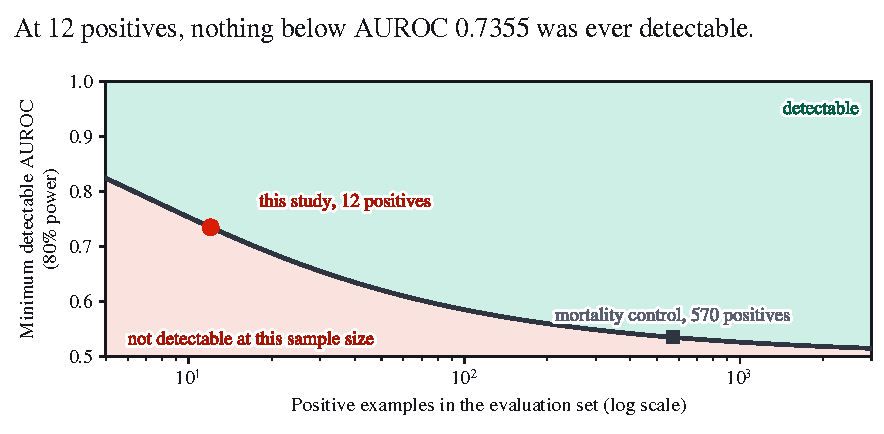
\includegraphics[width=0.98\linewidth]{figures/fig-power.pdf}
\label{fig:power}
\end{figure}

The minimum detectable AUROC comes from a formula this thesis has
already found unreproducible once (Appendix~\ref{app:corrections}, R9). A
Monte Carlo check, written for this thesis and released with it, draws
$5{,}000$ synthetic score sets at this evaluation's class counts ($12$
positives, $241$ negatives) from an equal-variance binormal calibrated to
each target AUROC and records how often a two-sided Mann-Whitney test at
$\alpha = 0.05$ rejects; its interpolated crossing of $80\%$ power, $0.7324$,
agrees with the analytic $0.7355$ to within three thousandths of an AUROC
point. Because its only inputs are the class counts, $\alpha$, and the target
grid, with no ACCORD score, gold label, or clinical data, this is a numerical
corroboration that $0.7355$ was computed correctly, not an empirical check on
the instrument. The claim that survives is the one the formula already
supported: the $253$-pair evaluation's null is informative about true AUROC
values at or above $0.7355$ and silent below that line.

\subsection{Multiplicity, and what is not corrected for}
\label{sec:r-multiplicity}

\textbf{No multiple-comparison correction is applied anywhere in this thesis.}
The single threshold every reported $p$ value in this chapter is read against
is the conventional $\alpha = 0.05$, uncorrected, and no result in this
chapter is described as surviving or clearing a correction it was never
subjected to. Sidedness is stated plainly rather than left implicit: the
Mann-Whitney tests of Table~\ref{tab:decontam}, the DeLong tests of
Table~\ref{tab:delong}, the mechanism Fisher test, the Welch test on the
anisotropy control, and the minimum-detectable-effect calculation of
Section~\ref{sec:res-rq4} are all two-sided; the local ambiguity-gradient
Fisher tests and the feasibility gate's attainable floor are one-sided,
because each bounds the most agreeable outcome a marginal permits; sidedness
for the Spearman correlations below is not recorded in the artifact behind
them. The gate's hypergeometric floors (Table~\ref{tab:feasgate}) are
preconditions, not members of this family: each is computable before a pair
is scored, so it bounds what a test could show rather than testing what was
observed. A correction record documents this history (C68, C76, C79, C85,
C88, C90, C92) rather than narrating it.

The tests this chapter still reports are enumerated in the committed register
released with the analysis code, one entry per test bound to the artifact and
key its $p$ value is read from; the withdrawal removed the eight frontier
Fisher exact tests, the four frontier Mann-Whitney tests, the four Bedrock
discrimination tests, and the eight hosted ambiguity-gradient tests, because
the runs behind every one of them are withdrawn (Section~\ref{sec:r-frontier}).
What remains is the five Mann-Whitney tests of Table~\ref{tab:decontam}, the
five DeLong tests of Table~\ref{tab:delong}, the one Fisher exact test on the
Rule 1/2 versus Rule 3/4 mechanism split (Section~\ref{sec:res-rq1}), the four
local Fisher exact tests on the ambiguity gradient
(Section~\ref{sec:r-ambiguity}), the one Welch two-sample $t$ test on the
anisotropy control, and four Spearman rank correlations against the
pharmacist's danger rating. No committed script has recomputed a family size
since the withdrawal, so none is typed here: the current count is in the
register.

A test belongs to this family by its inferential target, not by what a run
was commissioned for: two tests asking the same question of the same rows
count once regardless of which experiment produced the artifact, a
sensitivity analysis on a nested subset is a robustness check rather than a
second test, and a test whose target is this project's own bookkeeping, such
as the joinability check of Section~\ref{sec:r-exemplar}, is outside every
family (C90). No surviving block is close to independent: the five
Mann-Whitney tests are three seeds of one model, their ensemble, and one
further run, all on the same $253$ rows; the five DeLong tests are five
comparisons against a single reference run; and the four local ambiguity
tests are two models under two prompts each, scored on the same $46$
ambiguous and $241$ clear-negative pairs. The absence of a rejection across
any correlated block is weaker evidence than the same absence would be for a
single pre-specified test, and any single rejection inside one would be
correspondingly weaker evidence.

Two more Spearman tests against the same target are disclosed here rather
than left out silently: the contradiction-probability score against the
danger rating returns $\rho = -0.0286$ at $p = 0.6224$ over all $299$ pairs
and $\rho = -0.2771$ at $p = 0.3833$ over the $12$ positives, and the harm
score against the rating restricted to the $12$ positives returns
$\rho = -0.6621$ at $p = 0.019$, nominally below $0.05$ on twelve cases;
Section~\ref{sec:res-rq3} already reports the fourth, the harm score over all
$299$ pairs. None of the four is treated as evidence of anything, since the
harm head is already read as untrained and the contradiction-probability
score is this project's own detector rather than an external labeller;
reporting only the null members of a family the reader cannot see is the
defect this subsection exists to prevent.

\subsection{The positive control}

The remaining objection is that the apparatus, the training loop, the
splits, the seeds and the evaluation harness, cannot resolve any effect, and that
is answerable only by running the same apparatus where an effect is known to
exist. The control has a public arm, AG News, and a clinical arm built for
this control rather than for its own sake, in-hospital mortality predicted
from a patient's first 48 hours of notes, evaluated on $6{,}776$ held-out
admissions holding $570$ positives, a different task and cohort from
the $253$-pair contradiction evaluation. Four arms on the public task,
a pretrained encoder and three from-scratch encoders at different
pretraining scales, were each trained at 3, 6, 12 and 24 epochs, three seeds
per cell, for 48 runs and 555 minutes of compute. The adjudication rule
(Table~\ref{tab:m-prereg}) was committed before the sweep ran: a gap of at
least $3.0$ accuracy points between the pretrained arm and the best
from-scratch arm at the longest budget, with non-overlapping
one-standard-deviation bands, licenses reading the clinical null as measured;
a smaller or unresolved gap reverts it to an insensitivity finding; $2.5$ to
$3.5$ points is inconclusive in advance, and the rule forbids resolving that
by adding seeds.

\begin{table}[H]
\caption[Convergence sweep across training budgets]{Convergence sweep: four arms at four training budgets.}
\centering
\small
\begin{tabular}{lrrrr}
\toprule
\textbf{Arm} & \textbf{3 epochs} & \textbf{6 epochs} & \textbf{12 epochs} &
\textbf{24 epochs} \\
\midrule
Pretrained encoder & 0.9392 (0.0012) & 0.9369 (0.0004) & 0.9375 (0.0012) & 0.9379 (0.0029) \\
Scratch, 100M      & 0.8885 (0.0012) & 0.8903 (0.0034) & 0.8888 (0.0011) & 0.8925 (0.0004) \\
Scratch, 30M       & 0.8833 (0.0009) & 0.8856 (0.0035) & 0.8845 (0.0022) & 0.8886 (0.0015) \\
Scratch, 10M       & 0.8784 (0.0022) & 0.8795 (0.0013) & 0.8822 (0.0011) & 0.8838 (0.0036) \\
\bottomrule
\end{tabular}
\apanote{Accuracy, three seeds per cell, SD in parentheses; 48 runs, 555 minutes total, topic classification on AG News. The adjudication rule, committed at commit \texttt{b048829} before the sweep ran: Outcome A is a gap of at least $3.0$ points with disjoint SD bands; Outcome B is a gap below $3.0$ or an unresolved ordering; $2.5$ to $3.5$ is inconclusive in advance, and the rule forbids resolving that by adding seeds. Prose gaps use unrounded values, not these four-decimal cells, which can differ in the last digit.}
\label{tab:conv}
\end{table}

The gap between the pretrained arm and the best from-scratch arm is $5.07$ points
at 3 epochs and $4.53$ points at 24. Eight times the budget moved the pretrained
arm by $-0.13$ points and the 100M from-scratch arm by $0.41$. The gap did not
close, the arms had converged by the smallest budget in the sweep, and every cell
has a seed-to-seed standard deviation at or below $0.0036$. That is the harness
resolving a real effect on the public task; on the mortality control task the
same harness returns a gap of $0.0031$, reported next.

\begin{table}[H]
\caption[Pretraining gap versus parameter count]{Pretraining against parameter count, and the same contrast on the
mortality control task.}
\centering
\small
\begin{tabular}{llrr}
\toprule
\textbf{Task} & \textbf{Arm} & \textbf{Parameters} & \textbf{Score} \\
\midrule
Public benchmark  & Pretrained encoder & 85,648,132 & $0.9396 \pm 0.0010$ \\
Public benchmark  & Scratch, 100M      & 99,234,820 & $0.8878 \pm 0.0016$ \\
Public benchmark  & Scratch, 30M       & 31,913,860 & $0.8833 \pm 0.0009$ \\
Public benchmark  & Scratch, 10M       & 10,649,092 & $0.8790 \pm 0.0040$ \\
Mortality control  & BioMedBERT         &            & $0.7693 \pm 0.0102$ \\
Mortality control  & From scratch       & 10,638,720 & $0.7662 \pm 0.0073$ \\
Mortality control  & Gap, three seeds each &         & $+0.0031$ \\
Mortality control  & Gap, lineage-pinned seeds only & & $-0.0011$ \\
\bottomrule
\end{tabular}
\apanote{Public rows are accuracy at one budget; mortality rows are AUROC.
The from-scratch arm has more parameters than pretrained yet trails it by a
gap larger than the mortality gap. The $4.53$-point headline is Table~\ref{tab:conv}'s
pre-registered sweep, not this budget; no significance test exists for the
mortality gap, and the $4.53$-point test omits \texttt{equal\_var=False}, so
any $p$ is Student's, not Welch. The arms share no seed set (pretrained
$1,2,3$; scratch $0,1,2$): dropping seed $0$, lacking split lineage, gives a
two-seed mean of $0.7703$, flipping the sign to $-0.0011$.}
\label{tab:scaling}
\end{table}

The bag-of-words baseline outranking the neural configurations is not a real
ordering either: Table~\ref{tab:delong} cannot separate configurations four
points apart, and whatever gap the baseline shows over the neural
configurations, measured on the same 12 positives, sits inside that same
noise.

\section{Metrics Near the Base Rate}
\label{sec:res-metrics}

At 12 positives against 241 negatives the standard summary statistics do
something mechanical, and it is worth reporting apart from the system because it
is arithmetic and survives any change of system.

\subsection{The exchange rate}

Balanced accuracy \citep{brodersen2010balanced} is the unweighted mean of
sensitivity and specificity, so a classifier that forgoes one true positive is
preferred whenever it avoids more than $Q/P$ false positives, which on $G_{253}$
is $241/12$. Prevalence-adjusted bias-adjusted kappa \citep{byrt1993pabak} is an
affine transform of raw accuracy, so its rate is one avoided false positive per
forgone true positive, which at this base rate is more hostile to the minority
class than balanced accuracy rather than less, despite the name. Matthews
correlation \citep{matthews1975mcc} is not affine in the confusion cells and has
to be checked numerically. None of this is new
\citep{feinstein1990paradoxes,cicchetti1990resolving,delgado2019kappa}; this
chapter applies it to these class counts.

\subsection{The ordering and its intervals}
\label{sec:r-ordering}

\begin{table}[H]
\caption[Matthews correlation with bootstrap intervals]{Matthews correlation on the 253 non-ambiguous pairs.}
\centering
\small
\begin{tabular}{lrrr}
\toprule
\textbf{System} & \textbf{Predicted positive} & \textbf{MCC} & \textbf{95\% bootstrap CI} \\
\midrule
ACCORD at $\tau = 0.5$         & $11 + 223 = 234$ & $-0.0070$ & $-0.1626$ to $0.0753$ \\
Llama 3 8B evaluation baseline & $11 + 231 = 242$ & $-0.0436$ & $-0.2337$ to $0.0563$ \\
\bottomrule
\end{tabular}
\apanote{Cells from Table~\ref{tab:systems253}. The predicted-positive column
is shown as the sum of the two underlying cells. MCC is the statistic most
often recommended for imbalanced binary evaluation \citep{chicco2020mcc}, and
zero is chance. Intervals are percentile bootstraps at $B = 10{,}000$ and seed
42, resampling pairs with labels held fixed. Both rows contain zero. A
frontier-scale labeller was also scored on this set through a hosted API; that
row and its interval are withdrawn (Section~\ref{sec:r-frontier}) and do not
appear here.}
\label{tab:mcc}
\end{table}

The two systems this pipeline produced, ACCORD at $\tau = 0.5$ and the Llama 3 8B
evaluation baseline, differ from zero by less than $0.05$, and both 95 percent
bootstrap intervals contain zero (Table~\ref{tab:mcc}), overlapping over almost
their whole length. Figure~\ref{fig:forest} is that analysis in one view. No
claim in this thesis rests on the ordering between them.

Whether 12 positives could ever resolve a discrimination result at all is not a
question this table can answer on its own: an analysis that might have
addressed it directly was run through a hosted service and is withdrawn along
with every number computed from it. Neither system this pipeline produced,
ACCORD at $\tau = 0.5$ nor the Llama 3 8B evaluation baseline, is
distinguishable from chance on the 12 positives. This chapter does have one
local-only labeller row that is: \texttt{granite3.3:8b} zero-shot rejects the
null at a nominal, uncorrected one-sided hypergeometric $p$ of $0.0242$ on
$G_{253}$ and $0.0290$ on $G_{299}$ (Table~\ref{tab:feasgate}). That row also
sits exactly on its own ceiling, so a percentile-bootstrap MCC interval is not
a valid test of it on top of the hypergeometric one: at that flag rate almost
every resample still flags almost every confirmed case and so returns a
positive MCC, and no interval excluding zero for a row at
ceiling is evidence of anything the ceiling does not already guarantee.
The instrument's sensitivity to a real effect at this sample size is instead
established as in Section~\ref{sec:res-rq4}, on the mortality
positive control rather than on this task. The marginal feasibility gate of
Section~\ref{sec:r-feasgate} is the precondition a reader should apply to any
hard-label row before reading its agreement as evidence. It covers the
evaluation baseline (Table~\ref{tab:feasgate}), which could not have rejected
the null at any outcome; it was not run on the ACCORD row, so no ceiling claim
is made about that one. What the sample-size
reading never covered, and still does not, is a comparison
that lives on the $241$ clear negatives rather than on the 12 positives, and
over-calling, the headline finding of Section~\ref{sec:res-rq2}, is measured
there.

Figure~\ref{fig:forest}'s three unit families are not built from intervals of one
kind: the first two are percentile bootstraps at $B = 10{,}000$, while the two
rows of the third family are normal approximations on the difference of two
three-seed means, $g \pm 1.96\sqrt{s_a^2/3 + s_b^2/3}$, not bootstraps and not
the seed standard deviations Chapter~\ref{ch:results}'s $\pm$ convention refers
to; a $t$ critical value on four degrees of freedom would widen both by about
$42$ percent without changing which of them crosses zero.

\begin{figure}[!t]

\centering
\caption[Headline estimates against zero]{Every headline estimate with its
95\% interval, one panel per unit, each with its own scale and zero rule, so no
distance is comparable across panels. The two AUROC rows are different systems
on different sets, $G_{253}$ and $G_{134}$. The public-benchmark row is the
single-budget comparison of Table~\ref{tab:scaling}, not the $4.53$-point
convergence figure; the mortality row is its three-seed comparison.}
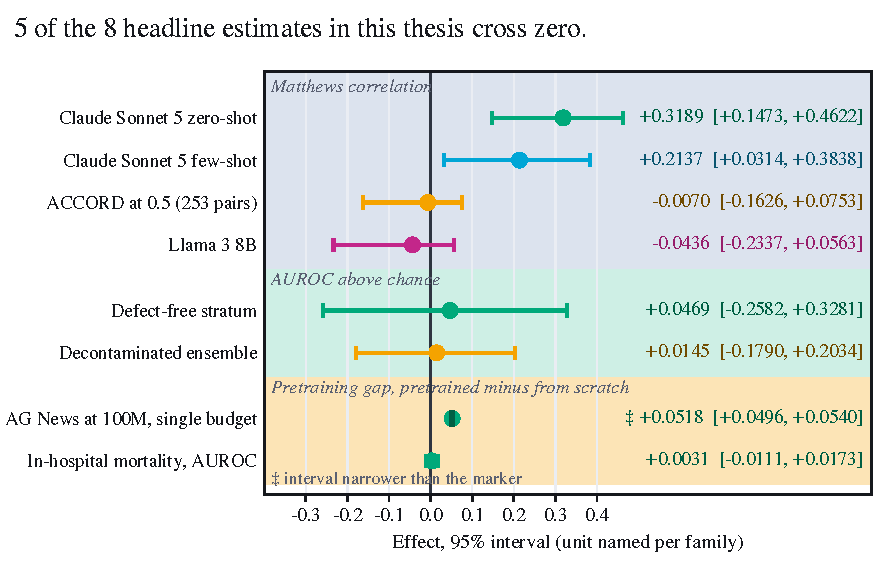
\includegraphics[width=0.98\linewidth]{figures/fig-forest.pdf}
\label{fig:forest}
\end{figure}

\subsection{Sign provenance}

Table~\ref{tab:signed} records the recomputation.

The three experiments in this subsection, the selection experiment and the two
PUMS regimes, run on simulated populations rather than the clinical pipeline,
and are retained because the sign-provenance rule they establish was
applied to the clinical numbers reported elsewhere in this thesis.

A second defect concerns direction rather than magnitude. Where a gap statistic
is stored as an absolute value, no directional claim can be recovered afterwards,
and a reader cannot tell which group a reported disparity favours. The signed
re-analysis reproduced the stored values exactly, at a maximum discrepancy of
$0.0$, which establishes that it is a faithful reproduction rather than a
different computation.

\begin{table}[H]
\caption[Signed parity endpoints, three experiments]{Signed demographic parity endpoints in three experiments.}
\centering
\small
\begin{tabular}{lrrl}
\toprule
\textbf{Experiment} & \textbf{Endpoint 1} & \textbf{Endpoint 2} &
\textbf{Sign changes} \\
\midrule
Selection experiment & $0.00841$  & $0.18939$  & none \\
PUMS, regime A       & $-0.13556$ & $-0.19435$ & none \\
PUMS, regime B       & $-0.11807$ & $-0.04101$ & none \\
\bottomrule
\end{tabular}
\apanote{Endpoint 1 is the signed gap at the weakest selection strength swept, Endpoint 2 at the strongest, not the sweep's extrema. On regime A the true minimum and maximum, $-0.20733$ and $-0.12761$, both lie outside the printed endpoints; on regime B the true minimum, $-0.12034$, is more extreme than the printed $-0.11807$, while the true maximum coincides with it. On the selection experiment both printed endpoints are the sweep's own extrema. All endpoints are reported as recorded.}
\label{tab:signed}
\end{table}

The sign analysis establishes that absolute-value storage destroys the
information a directional claim needs and that the three experiments
re-examined do not change sign inside their own sweeps; it demonstrates no
harm to any subgroup, and with 12 positives no subgroup performance claim is
supportable.

\section{Practice}
\label{sec:res-rq5}

Does the field run the checks that would have caught the failures above? This
section reports a prevalence measurement on a deliberately enriched corpus, not
a finding of the same standing as the ablation in
Section~\ref{sec:res-rq3} or the pre-registered positive control in
Section~\ref{sec:res-rq4}. It is reported because a prevalence measurement on
its own terms is worth having, and because the survey coding table of Appendix~\ref{app:survey} makes
the full 75-paper coding available for a reader to check rather than take on
trust. Of the $525$ coded fields, $502$ carry a verbatim quote checked by exact string match
against the source text, so no coded value asserting a property of a paper survives without
verified textual support. The remaining $23$ are codings of absence, recording that a paper does
not mention how it handles null attribute values; there is no sentence to quote for an absence,
and those $23$ are the \emph{not mentioned} row of Table~\ref{tab:survey}. A systematic coding of 75 papers says: rarely on the strict
reading, and not much more often on the permissive one. Both are reported side by side; the
choice between them is a judgement call for the reader.

\subsection{Both readings, and the null-attribute distribution}

\begin{table}[H]
\caption[Coded outcomes across surveyed papers]{Coded outcomes across 75 included papers.}
\centering
\small
\begin{tabular}{lr}
\toprule
\textbf{Coded outcome} & \textbf{Papers} \\
\midrule
Runs a model over the candidate pool  & 75 \\
Reports the check, permissive reading & 14 \\
Reports the check, strict reading     & 4  \\
\midrule
\multicolumn{2}{l}{\textit{Handling of null attribute values}} \\
Not mentioned     & 23 \\
Drops the rows    & 17 \\
Separate category & 13 \\
Unclear           & 9  \\
Imputes           & 7  \\
Reports only      & 6  \\
\bottomrule
\end{tabular}
\apanote{Papers are coded once each; the denominator is 75 throughout. The first row is the screening condition, satisfied by every included paper by construction. The permissive reading accepts any statement that the check was performed; the strict reading requires the quantity that would make it verifiable. The six null-attribute categories are exclusive and sum to 75.}
\label{tab:survey}
\end{table}

Four of 75 papers report the check under the strict reading and 14 under the
permissive one, so 61 report it under neither. The 10-paper gap between the two
readings is the population that says it did the check without reporting what the
check returned, and the strict count is the one a reader can verify. Twenty-three
papers, the largest single category, do not mention the null-attribute question
and nine more are coded unclear, so 32 of 75 give a reader no way to tell what
happened to rows with a missing attribute. Dropping and imputing are not
equivalent and neither is neutral, and the two choices move a reported disparity
in different directions; 17 papers take the first and 7 the second. The point is
not that one choice is wrong; it is that 32 of 75 leave it unrecoverable.

\subsection{Reliability}

One coder coded all 75 papers under the shared written rule set described in
Chapter~\ref{ch:method}. A blind second coder independently re-coded a
19-paper subsample, given the field definitions but not the hypothesis, and
that subsample is the basis for every agreement figure in this section; no
agreement is claimed for the remaining $75 - 19 = 56$ papers, which were coded
once. On the permissive cell agreement is $0.9474$ and Cohen's kappa is
$0.855$; on the
null-attribute-handling coding agreement is $0.7895$ and kappa is $0.730$.

The strict cell has no defined agreement coefficient, for a structural
reason: chance-corrected agreement
\citep{cohen1960kappa} is a ratio whose denominator is one minus expected
agreement, and when a coder's marginal on a category is degenerate that
denominator goes to zero and the coefficient is undefined rather than perfect. At
4 positive codes in 75 the strict cell is degenerate on the double-coded
subsample specifically: on the 19 overlap papers neither coder found a
strict-positive paper, so agreement is $1.0$ but kappa is undefined rather
than perfect. Reporting perfect agreement as a defined kappa would be exactly
the error the statistic exists to prevent.

The corpus is enriched, and the enrichment runs against the finding rather
than for it: a corpus that over-samples work already attentive to these
questions still yields 4 of 75 strictly, which bounds the bias without
turning 75 papers into a population estimate for the field.
